\documentclass{article}

\usepackage[utf8]{inputenc}
\usepackage[margin=1.1in]{geometry}
\usepackage[parfill]{parskip}
\usepackage{algorithm}
\usepackage[noend]{algpseudocode}
\usepackage{amsmath}
\usepackage{amssymb}
\usepackage{graphicx} 
\usepackage[font=small]{caption}
\usepackage{subcaption} 

\graphicspath{{./imgs/}}


\title{Converting Q-trees to a decision tree}
\author{Andreas Holck Høeg-Petersen}


\begin{document}

\maketitle

\section{Q-trees}

A Q-tree is a binary tree that represents a complete partition of a
$k$-dimensional (state) space according to a learned set of Q-values for a given
action in a Reinforcemnt Learning setting. This means, a Q-tree is essentially a
replacement for the part of a Q-table that describes one single action. A
collection of Q-trees, a Q-forest, that covers all the possible actions is
therefore a complete replacement for a Q-table.

The nodes in a Q-tree each give a linear partition of the state space with
respect to a certain variable $X$. The node $n_i$ compares $X$ to some bound
$b_i$ and hosts a subtree for states with $X \leq b_i$ and one for $X_i > b_i $.
At the leafs, the Q-value for that particular evaluation of the state for a
specific action is stored. Each leaf therefore represents not only a Q-value and
an action, but also an area of the state space with well-defined bounds. 

An example of Q-forest is given in Figure~\ref{fig:QForest}. This describes a
strategy for a (fictive) setting, where there are three allowed actions,
$\alpha, \beta \text{ and } \gamma$, and two variables to account for, $var_1
\text{ and } var_2. $

\begin{figure}[ht]
    \centering
    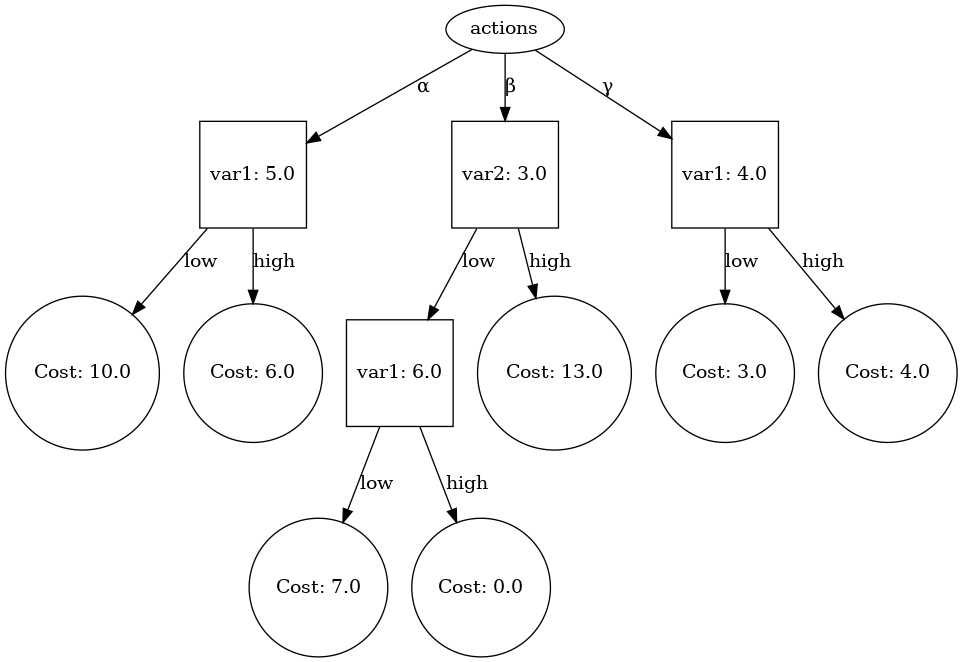
\includegraphics[width=.8\textwidth]{exampleQTree}
    \caption{%
        An example of a Q-forest with three actions and two variables.
    }\label{fig:QForest}
\end{figure}


\section{Notation}

Let $\mathcal{L} = \{ L_1, L_2, \ldots, L_n \}$ be the set of all leaves in a
Q-forest, let $\mathcal{A} = \{ A_1, A_2, \ldots, A_m \}$ be the set of all
possible actions and let $\mathcal{V} = \{ V_1, V_2, \ldots, V_k \}$ be the $k$
observable variables in the environment (where $V_i \in \mathbb{R}$ for all
$i=1\ldots k$). For any $L_i \in \mathcal{L}$, we can define a state partition
$S_i = \{ (l_{i,1}, u_{i,1}), (l_{i,2}, u_{i,2}), \ldots, (l_{i,k}, u_{i,k})\}$
where $u_{i,j}$ is the \textit{upper} bound for the value of variable $V_{j}$ at
the leaf $L_i$ and $l_{i,j}$ is the \textit{lower} bound. We consider all
variables to ultimately be bounded by either positive or negative infinity,
meaning that if no smaller bound is given $u_{i,j} = \infty$ and $l_{i,j} =
-\infty$.

Now we can define a leaf $L_i$ as a triplet of $(a_i, q_i, S_i)$ where $a_i \in
\mathcal{A}$ is the action associated with the Q-tree to which the leaf belongs,
$q_i \in \mathbb{R} $ is the expected Q-value and $S_i$ is the state partition
that the leaf covers. Notice that we do not actually care about the original
trees nor the internal nodes of these trees. All the information relevant to our
purpose is contained in $\mathcal{L}$, the complete set of leaves in the forest.

As an example of an actual leaf, the `left-most' leaf in the Q-forest in
Figure~\ref{fig:QForest} can be described by the triplet $(\alpha, 10, \{
(-\infty, 5), (-\infty, \infty)\})$, assuming that $V_1 = var_1$ and $V_2 =
var_2$.\looseness=-1

\section{The algorithm}

The goal is to take all the leafs of a Q-forest and from these build a single
binary decision tree, that through evaluation of a state arrives at a leaf node
indicating the best action to take. The general idea of the algorithm is to
repeatedly take the next leaf $L_i$ in $\mathcal{L}$, which we (because of our
sorting) know to have the best Q-value, and insert its action into the decision
tree we are building so that it respects $S_i$. This means, that the internal
nodes of the tree will still be checks on variables in $\mathcal{V}$.

\subsection{Creating the root}

We initialise the tree from the lowest valued leaf in $\mathcal{L}$ which we
will denote $L_0$. The operation of inserting $L_0$ into the at this point empty
tree requires special attention, since we have to create split nodes for all the
variable bounds $(l_{0,i}, u_{0,i})$ in $S_0$. We denote this operation
\texttt{MakeRoot} and its pseudocode is given in Algorithm~\ref{alg:MakeRoot}.

\begin{algorithm}[ht]
    \caption{MakeRoot}\label{alg:MakeRoot}

    \begin{algorithmic}[1]
        \Procedure{MakeNewNode}{$var, bound, action, isHigh, prevNode$}
            \State{$node \gets \texttt{Node}(var, bound)$}
            \If{isHigh}
                \State{$node.high \gets \texttt{Leaf}(action, \infty, \texttt{State}(\cdot))$}
            \Else%
                \State{$node.low \gets \texttt{Leaf}(action, \infty, \texttt{State}(\cdot))$}
            \EndIf%

            \If{$prevNode \text{ is not } \texttt{None}$}
                \If{$prevNode.low \text{ is } \texttt{None}$}
                    \State{$prevNode.low \gets node$}
                \Else%
                    \State{$prevNode.high \gets node$}
                \EndIf%
            \EndIf%
            \State{$\mathbf{return}\quad node$}
        \EndProcedure%
        \item[]%
    \end{algorithmic}

    \begin{algorithmic}[1]
        \Function{MakeRoot}{$\texttt{Leaf}(a_0, q_0, S_0)$}

        \State{$rootNode \gets \texttt{None}$}
        \State{$prevNode \gets \texttt{None}$}
        \For{$(l_{0,i}, u_{0,i}) \text{ in } S_0$}
            \If{$u_{0,i} < \infty$ }
                \State{$prevNode \gets \text{\Call{MakeNewNode}{$V_i, u_{0,i}, a_0, \texttt{True},
                        prevNode$}}$}%
                \If{$rootNode \text{ is }\texttt{None}$ }
                    \State{$rootNode \gets prevNode$ }
                \EndIf%
            \EndIf%

            \If{$l_{0,i} > -\infty$ }
                \State{$prevNode \gets \text{\Call{MakeNewNode}{$V_i, l_{0,i},
                    a_0, \texttt{False}, prevNode$}}$}%
                \If{$rootNode \text{ is }\texttt{None}$ }
                    \State{$rootNode \gets prevNode$ }
                \EndIf%
            \EndIf%

        \EndFor%

        \If{$prevNode.low \text{ is }\texttt{None}$ }
            \State{$prevNode.low \gets \texttt{Leaf}(a_0,q_0,S_0)$ }
        \Else%
            \State{$prevNode.high \gets \texttt{Leaf}(a_0,q_0,S_0)$ }
        \EndIf%
        \State{$\mathbf{return}\quad rootNode$ }
        \EndFunction%
    \end{algorithmic}

\end{algorithm}

The operation iterates through all tuples $(u_{0,i},l_{0,i})$ in $S_0$ and
whenever it encounters a bound that is different from the limit (which we here
assume to be infinity) it has to insert a new node into the tree. This is done
via the \texttt{MakeNewNode} procedure, which we define as a helper function to
avoid repetitions in the algorithm. This function takes the variable $V_i$ that
the encountered bound relates to, the value of the bound and the action of the
leaf, we are inserting. It then creates a new internal node, that represents
the partition according to the inequality $V_i \leq b$ where $b \in (u_{0,i},
l_{0,i})$.

Now, \texttt{MakeNewNode} also takes two additional arguments, one boolean to
indicate if the bound is an upper bound or not and the current parent node
(which might be \texttt{None}). If the bound is an upper bound, then we know
that $Q(a_0) = q_0$ only holds if $V_i \leq u_{0,i}$. This means, that $L_0$
should be inserted somewhere in the left (`low') subtree of the newly created
node, while the right (`high') subtree should for now just be set to some
random leaf with a very poor Q-score (we will find better values for these
subtrees when we process the remaining leaves of $\mathcal{L}$).

Lastly, if the current parent node is not \texttt{None}, then we know it has one
subtree that is set (like above) and one that itself is \texttt{None} as it is
reserved for our newly created node. We therefore set the undefined child of the
parent node to our new node and returns this new node, which is then marked as
being the new parent node. If this our first new, we also mark it as our root
node.

When we have processed all the bounds in $S_0$, we insert $L_0$ at the `free'
spot in the parent node and return the root node. With this approach, we end up
with an initial tree that is very shallow and basically only has one interesting
leaf at the maximum depth of the tree. An example of this is given in
Figure~\ref{fig:rootTree}, where we have built the root tree from the leaf
defined by $\texttt{Leaf}(\beta, 7, \{ (-\infty, 6), (-\infty, 3) \})$.

\begin{figure}[ht]
    \centering
    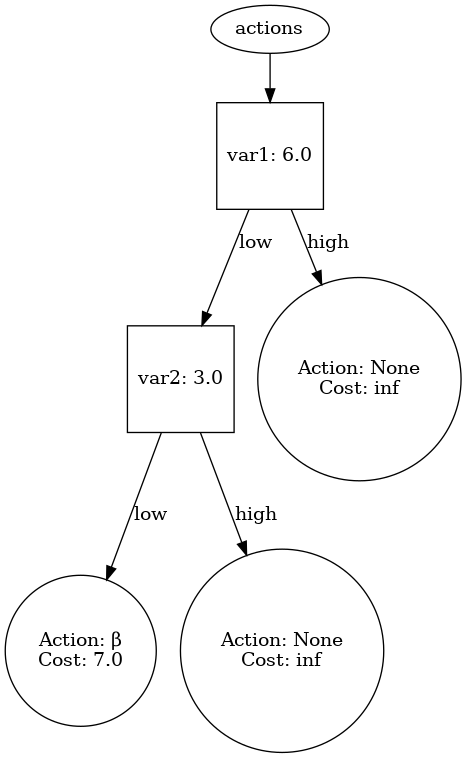
\includegraphics[scale=0.4]{exampleRoot}
    \caption{%
        Tree build using \texttt{MakeNewNode} and the leaf triplet $(\beta, 7,
        \{ (-\infty, 6), (-\infty, 3) \})$ 
    }\label{fig:rootTree}
\end{figure}

\subsection{Inserting the leaves}

To insert the remaining leaves we need a couple of extra helper functions. The
task is to identify or construct all the paths in the tree under construction
that leads to leaf nodes where the action of the leaf that are being inserted is
to be preferred.

When we insert $L_i = (a_i, q_i, S_i)$, we will always either encounter an
internal branch node that defines a split on a variable and has two subtrees, or
we encounter a leaf node storing an action, a Q-value and a state partition. We
therefore define a general \texttt{Put} function (Algorithm~\ref{alg:putAll}),
that takes a root node and a leaf triplet to be inserted and decides what to do based
on the type of the root node (either a branch node or a leaf node).

\begin{algorithm}[ht]
    \caption{Build decision tree from leaves of Q-tree}\label{alg:putAll}.

    \begin{algorithmic}[1]
        \Function{Put}{$root, \texttt{Leaf}(a, q, S)$ }
        \If{$root \text{ is } \texttt{Node}$}
            \State{$\mathbf{return }\quad \text{\Call{PutAtBranchNode}{$root,
                        \texttt{Leaf}(a,q,S)$} }$}
        \Else\Comment{$root$ is a \texttt{Leaf}}%
            \State{$\mathbf{return}\quad \text{\Call{PutAtLeafNode}{$root,
                \texttt{Leaf}(a,q,S)$}}$}
        \EndIf%
        \EndFunction%
    \end{algorithmic}

\end{algorithm}

We will first deal with situation where we encounter an internal node, $N_j$,
which splits on variable $V_k$ at bound $b$. We now need to check on what side
of this split $S_i$ falls (it might be both). So we test on both $u_{i,k} > b$
and $l_{i,k} < b$. If the first check is true, then we know that $S_i$ defines
an area for $V_k$ that can be larger than $b$, why we have to visit the right
(`high') subtree of $N_j$. Likewise for the latter test, only then we have to
continue our insertion in the left (`low') subtree. Note that both tests
can be true.\looseness=-1

We do, however, need to keep track of the implicit limitations we put on $S_i$
as we go along. When continuing our insertion of $L_i$ in the subtree of $N_j$
defined by $V_k > b$, then we should reflect in $S_i$ that now $V_k$ has a lower
bound $b$, that is, we should set $l_{i,k} = b$. We do this in the algorithm
through an implicit helper function \texttt{SetLower$(state, var, bound)$} (and
likewise \texttt{SetUpper} for updating the upper bound). The pseudocode for
this is given in Algorithm~\ref{alg:putInternal}.

\begin{algorithm}[ht]
    \caption{PUT Q-leaf into an internal node}\label{alg:putInternal}

    \begin{algorithmic}[1]
        \Function{PutAtBranchNode}{$\texttt{Node}(V_k, b, low, high),
            \texttt{Leaf}(a_i, q_i, S_i)$ }%
            
        \If{$l_{i,k} < b$}
            \State{$S'_i \gets \text{\Call{SetUpper}{$S_i, V_k, b$}}$}
            \State{$low \gets \text{\Call{Put}{$low, \texttt{Leaf}(a_i, q_i,
                        S'_i)$}}$}
        \EndIf%
        \If{$u_{i,k} > b$}
            \State{$S'_i \gets \text{\Call{SetLower}{$S_i, V_k, b$}}$}
            \State{$high \gets \text{\Call{Put}{$high, \texttt{Leaf}(a_i, q_i,
                        S'_i)$}}$}
        \EndIf%

        \State{$\mathbf{return}\quad \texttt{Node}(V_k, b, low, high)$}
        \EndFunction%

    \end{algorithmic}

\end{algorithm}

The second case is when we encounter a leaf node during the insertion operation.
We denote this node as $L_t$ to indicate that it is a leaf already present in
the tree under construction. First, we check if the Q-value of $L_t$ is better
than that of $L_i$, in which case we do nothing and abort the insert operation.
If $q_i$ on the other hand is the better option, then we need to insert $L_i$
but in a way that respects $S_i$.\looseness=-1

It is guaranteed at this stage, that $S_t$ contains $S_i$, that is $u_{t,j} \geq
u_{i,j}$ and $l_{t,j} \leq l_{i,j}$ for all $j=1,2,\ldots,k$. But this also
means that in the cases where the bounds on $S_t$ are strictly larger or smaller
than those of $S_i$ then we need to insert a new internal node to ensure this
partition before we can insert $L_i$. In other words, if $u_{t,j} > u_{i,j}$,
then we need to create a branch node that splits on $V_j$ at bound $b =
u_{i,j}$ and whose right (`high') subtree is the original leaf $L_t$ but with an
updated state $S_t$ where $l_{t,j} = u_{i,j}$. The left (`low') subtree should
also, for a start, be set to $L_t$ but then we continue the insert operation on
this side, either creating more branch nodes or eventually inserting $a_i$ and
$q_i$ in place of $a_t$ and $q_t$.

The pseudocode for the function is given in Algorithm~\ref{alg:putLeaf}.

\begin{algorithm}[h!]
    \caption{Put Q-leaf into a leaf node}\label{alg:putLeaf}

    \begin{algorithmic}[1]
        \Procedure{Split}{$action, q, var, bound, state$}
            \State{$highState \gets \text{\Call{SetLower}{$state, var, bound$}}$}
            \State{$lowState \gets \text{\Call{SetUpper}{$state, var, bound$}}$}
            \State{$high \gets \texttt{Leaf}(action, q, highState)$}
            \State{$low \gets \texttt{Leaf}(action, q, lowState)$} 
            \State{$\mathbf{return}\quad \texttt{Node}(var, bound, low, high)$ }
            \item[]
        \EndProcedure%
    \end{algorithmic}

    \begin{algorithmic}[1]
        \Function{PutAtLeafNode}{$\texttt{Leaf}(a_t, q_t, S_t), \texttt{Leaf}(a_i, q_i, S_i)$}
        \If{$q_t \leq q_i$ }
            \State{$\mathbf{return}\quad \texttt{Leaf}(a_t, q_t, S_t)$}
        \EndIf%
        \item[]

        \For{$(l_{t,j}, u_{t,j}) \text{ in } S_t$}
            \If{$l_{t,j} < l_{i,j}$}
                \State{$newNode \gets \text{\Call{Split}{$a_t, q_t, V_j,
                            l_{i,j}$}}$}
                \State{$\mathbf{return}\quad
                    \text{\Call{Put}{$newNode, \texttt{Leaf}(a_i,
                            q_i, S_i)$}}$} 
                \item[]
            \ElsIf{$u_{t,j} > u_{i,j}$}
                \State{$newNode \gets \text{\Call{Split}{$a_t, q_t, V_j,
                            u_{i,j}$}}$}
                \State{$\mathbf{return}\quad
                    \text{\Call{Put}{$newNode, \texttt{Leaf}(a_i,
                            q_i, S_i)$}}$} 
            \EndIf%
            \item[]

        \EndFor%

        \State{$\mathbf{return}\quad \texttt{Leaf}(a_i, q_i, S_i)$}
        \EndFunction%
    \end{algorithmic}

\end{algorithm}

\subsection{Example}

Using this algorithm, we can now construct a decision tree from the Q-forest we
saw in Figure~\ref{fig:QForest}. For simplicity, we will simply consider the
obvious order of the leafs that comes from collecting them from left to right in
the figure, that is, we create our root from $\texttt{Leaf}(\alpha, 10, \{
(-\infty, 5), (-\infty, \infty) \})$ and the final input to \texttt{Put} is
$\texttt{Leaf}(\gamma, 4, \{ (4, \infty), (-\infty, \infty) \})$. Note that we
omit the step where we would insert $\texttt{Leaf}(\beta, 13, \{ (\infty,
-\infty), (3, \infty) \})$, as this has such a bad Q-value that it is just
discarded.

    
\section{Optimization}

When looking at the final tree in Figure~\ref{fig:traceComplete}, it is obvious
that it is not the most compact version of that tree. That is because we have
just inserted the leafs in a random order (the order of visual appearance in
Figure~\ref{fig:QForest}) and there is no attempt at restructuring or balancing
the tree during or after construction. Since the algorithm does not guarantee
optimality it is crucial in order to obtain acceptable results that we perform
some optimization steps before and after constructing the tree.

\begin{figure}[H]
    \centering
    \caption{%
        Complete trace of converting the Q-tree in Figure~\ref{fig:QForest} to
        a single decision tree.
    }\label{fig:traceComplete}
    \begin{subfigure}[t]{0.31\textwidth}
        \centering
        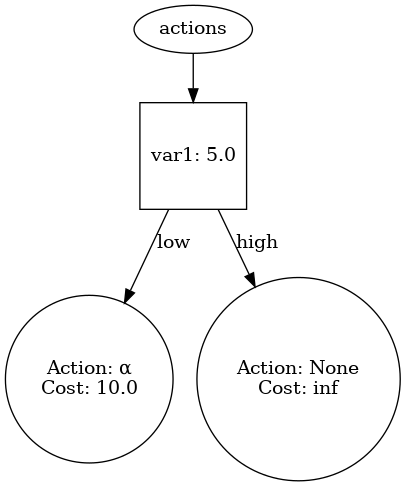
\includegraphics[width=.8\textwidth]{exampleBuild0}
        \captionsetup{labelformat=empty}
        \caption{%
            \texttt{MakeRoot}$(\alpha, 10, \{ (-\infty, 5),
            (-\infty, \infty) \})$
        }
        \vspace{3ex}
    \end{subfigure}
    \begin{subfigure}[t]{0.3\textwidth}
        \centering
        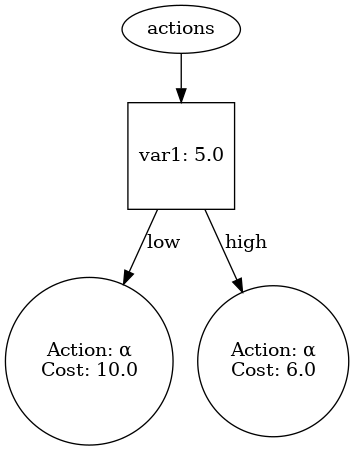
\includegraphics[width=.8\textwidth]{exampleBuild1}
        \captionsetup{labelformat=empty}
        \caption{%
            \texttt{Put}$(\alpha, 6, \{(5, \infty),(\infty,-\infty)\})$
        }
    \end{subfigure}
    \begin{subfigure}[t]{0.3\textwidth}
        \centering
        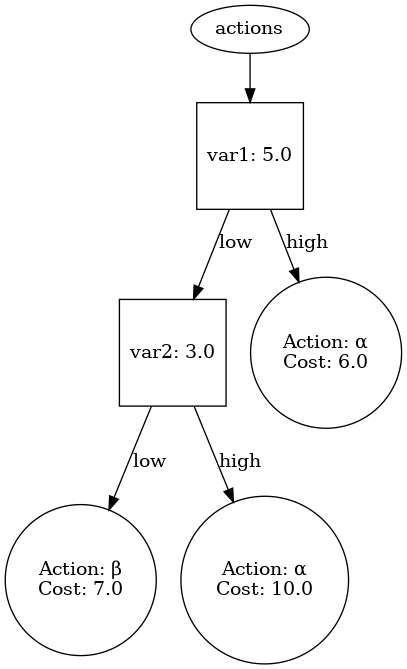
\includegraphics[width=.8\textwidth]{exampleBuild2}
        \captionsetup{labelformat=empty}
        \caption{%
            \texttt{Put}$(\beta, 7, \{(-\infty, 6),(3,-\infty)\})$
        }
    \end{subfigure}
    \begin{subfigure}[t]{0.35\textwidth}
        \centering
        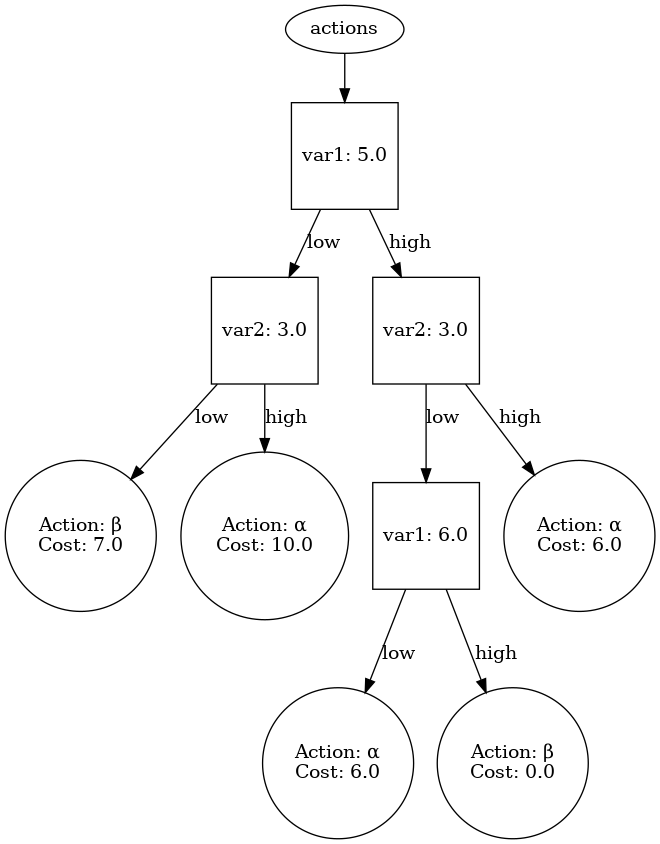
\includegraphics[width=.9\textwidth]{exampleBuild3}
        \captionsetup{labelformat=empty}
        \caption{%
            \texttt{Put}$(\beta, 0, \{(6, \infty),(3,-\infty)\})$
        }
        \vspace{2ex}
    \end{subfigure}
    \begin{subfigure}[t]{0.55\textwidth}
        \centering
        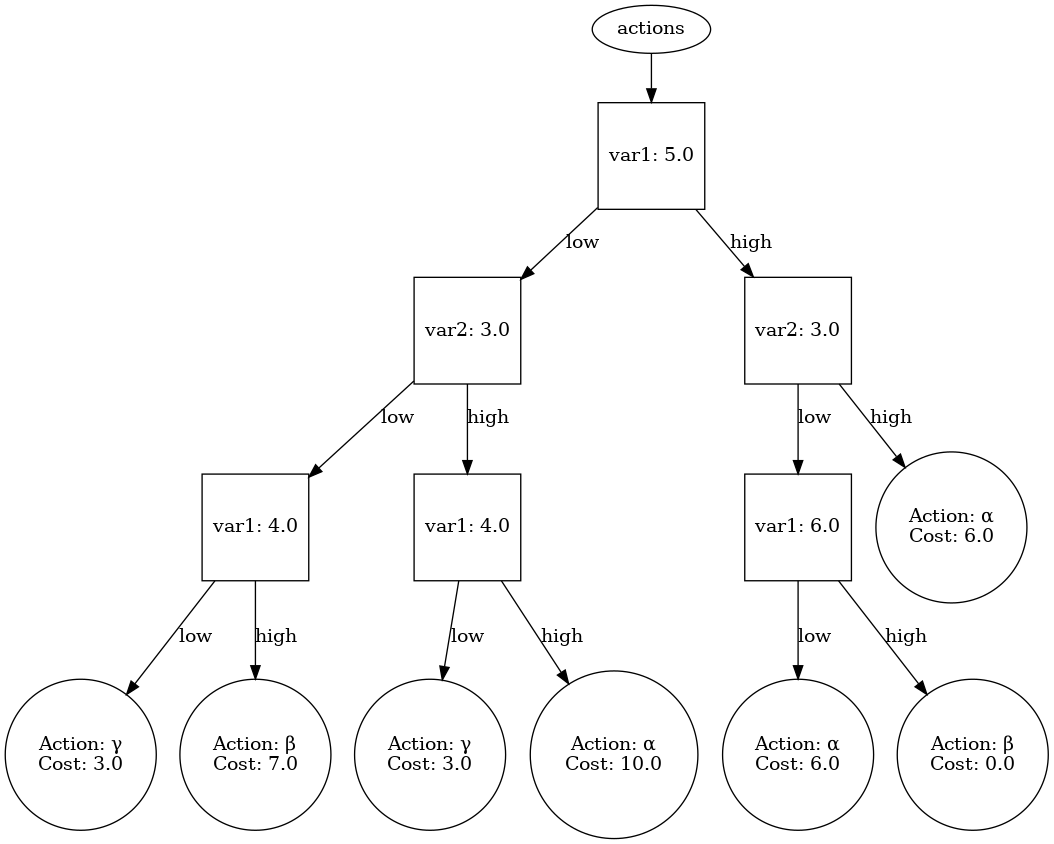
\includegraphics[width=.9\textwidth]{exampleBuild5}
        \captionsetup{labelformat=empty}
        \caption{%
            \texttt{Put}$(\gamma, 3, \{(-\infty, 4),(\infty,-\infty)\})$
        }
    \end{subfigure}
    \begin{subfigure}[t]{0.55\textwidth}
        \centering
        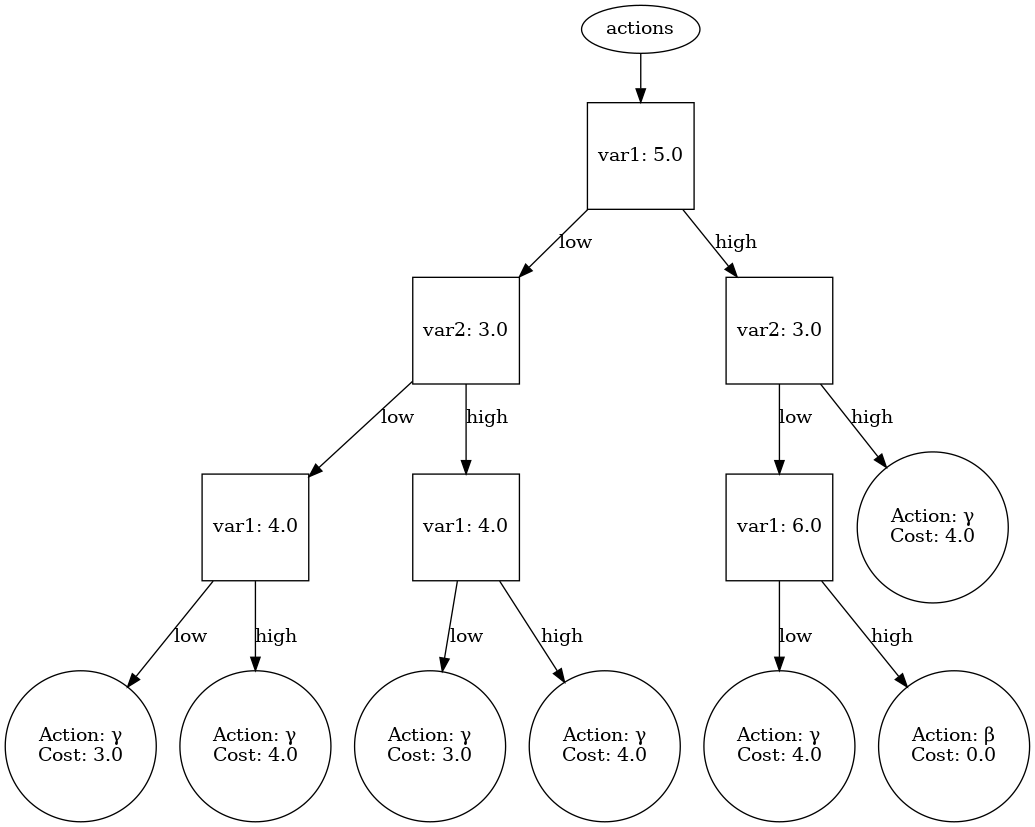
\includegraphics[width=.9\textwidth]{exampleBuild6}
        \captionsetup{labelformat=empty}
        \caption{%
            \texttt{Put}$(\gamma, 4, \{(4, \infty),(\infty,-\infty)\})$
        }
    \end{subfigure}
\end{figure}

First of all, the order in which we insert the leafs into the tree has a great
influence on the final size of the tree. This comes from the fact, that branch
nodes are created whenever the insert operation reaches a leaf that has a worse
Q-value than the one that is being inserted and where the state of the leaf is
not yet completely determined by the parent nodes. Therefore, if we sort
$\mathcal{L}$ in ascending according to the Q-values of the leaves, such that
for any two $q_i$, $q_{i+1}$ it holds that $q_i \leq q_{i+1}$\footnote{%
    This expects the Q-values to represent \textit{cost} values rather than
    \textit{rewards}. If the latter is the case, the inequality should be
    reversed.
} we will increase the likelihood that the tree structure is built in
service of the best leaf nodes rather than accommodating for the states of
sub-par leaves inserted earlier.

Secondly, as another pre-processing step, we prune any leaves $L_i$ for which
there exist a leaf $L_j$ such that $q_j \leq q_i$ and $S_j$ completely contains
$S_i$ (in which case, we say that $L_j$ dominates $L_i$). When $\mathcal{L}$ is
sorted, this is simply a matter of traversing $\mathcal{L}$ backwards and
comparing each $S_{i}$ with $S_{i-1}$. This does not have an effect on the final
tree if $\mathcal{L}$ has been sorted before insertion, but it will reduce the
size of $\mathcal{L}$ and possibly reduce the build time of the tree.

Lastly, after the tree has been built, we can perform another pruning operation.
In this, we search for branch nodes whose two children are both leaf nodes and
both have the same action. Since we --- for the purpose of using the tree to
decide on an \textit{action} given a state --- do not care about the actual
expected cost of the action, we can merge the two leaf nodes into one and
replace their common parent node with it. Doing this iteratively can greatly
reduce the size of the tree and not least the complexity of the strategy (when
viewed in a RL context). For example, if we look at the final tree of
Figure~\ref{fig:traceComplete}, we see that we could actually collapse the
entire left subtree into a single leaf nodes telling us to choose action
$\gamma$. This tells us, that as long as $var_1 \leq 5$ the best action to
choose is $\gamma$ which is a very easily interpretable strategy.

Applying all of these steps can result in significantly smaller trees. In
Figure~\ref{fig:optimalExample} the complete strategy originally shown as a
Q-forest in Figure~\ref{fig:QForest} is presented as a decision tree build
using all the techniques described in this section.

\begin{figure}[ht]
    \centering
    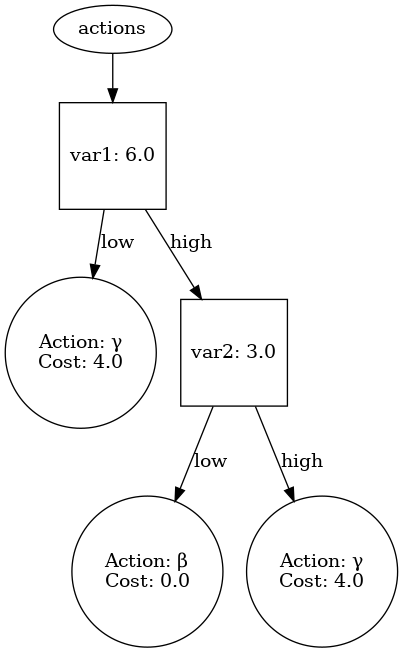
\includegraphics[scale=0.4]{exampleOptimal}
    \caption{%
        The complete Q-forest of Figure~\ref{fig:QForest} represented as a
        compact decision tree.
    }\label{fig:optimalExample}
\end{figure}

\subsection{Further optimization}

Beyond pre- and post-processing steps, we can also make improvements during
construction.

\section{Example of HOFOR case}

\subsection{Test for equivalence}

\subsection{Safety analysis}

\end{document}
